
%%% Local Variables: 
%%% mode: latex
%%% TeX-master: "digital_comm"
%%% End: 

\documentclass[onecolumn,x11names,technote,twoside,a4paper,12pt,english]{IEEEtran}
\usepackage[english]{babel}
\usepackage[pdftex]{graphicx}
\usepackage{amssymb}
\usepackage{amsmath}
\usepackage{caption}
\usepackage{float}
\usepackage{tikz}
\usepackage{euler}                                %Nicer numbers
\usepackage{listings}
\usepackage{subfigure}
\usepackage[shell,pdf]{dottex}

\newtheorem{example}{Example}

\begin{document}


\title{Introduction to Digital Communications Systems}
\author{Notes from lectures given by Lev~Goldfeld, summarized by Noam~Lewis [noamle@bgu.ac.il]}

\maketitle
\clearpage
\section{Introduction}
This report is about  digital communication systems (DCS). In the context of this report, a DCS is responsible for communicating digital information (bits) from transmitter to receiver, over an analog channel. The main issues that such a system must solve are:
\begin{enumerate}
\item Encoding of the digital information into an analog signal (encoder and transmit filter)
\item Transmission of the encoded (analog) signal over a noisy band-limited channel (modulator)
\item Receiving the analog signal  (linear section and demodulator)
\item Decoding the detected signal, with minimal loss of digital information (receive filter, decision device and decoder)
\end{enumerate}

\begin{figure}[h!]
  \centering
  \begin{dotpic}[width=2in]
    rankdir=LR; 
    input->DCS [label="bits\nsent"];
    DCS->output [label="bits\nreceived"];
    DCS [shape="box"];
    input [style="invisible"];
    output [style="invisible"];
  \end{dotpic}
  \label{fig:DCS}
\end{figure}

In this report we shall deal exclusively with additive, white gaussian noise channels (AWGN channels). Additive means that the received signal can be expressed as a sum of the transmitted signal and the noise. The gaussian white noise property eases analysis in general, and specifically of how the noise is affected when passing through elements of the receiver.

We shall touch on three types of systems:
\begin{enumerate}
\item Single-carrier
\item Multi-carrier
\item Spread spectrum
\end{enumerate}
The report is written so that subjects are gradually presented, so that each section builds on knowledge from previous ones.

\section{Single Carrier Systems}
\label{sec:single-carrier}

The input to a DCS is always a sequence of bits, denoted $\bar{b}$. On the receiving side the output of the system is another (ideally identical) sequence of bits, $\bar{b_r}$. The \emph{bitrate} of a DCS is the number of bits communicated per second, and is denoted $R_b$ (units: $\frac{\text{bits}}{\text{sec}}$).

\subsection{Transmitter}
\label{sec:sc-trans}

\begin{figure}[h!]
  \centering
  \begin{dotpic}[width=5in]
    rankdir=LR; 
    input->SE [label="bits"];
    SE->TF [label="symbols"];
    TF->Modulator [label="analog signal"];
    Modulator->output [label="modulated\nanalog signal"];
    TF [label="Transmit\nFilter",shape="box"];
    SE [label="Symbol\nEncoder",shape="box"];
    Modulator [shape="box"];
    input [style="invisible"];
    output [style="invisible"];
  \end{dotpic}
  \caption{General structure of a digital transmitter}
  \label{fig:DCS-Trans}
\end{figure}

As a first step, the bits in the sequence $\bar{b_r}$ entering a transmitter are encoded into symbols. The symbols are complex values (elements of $\mathbb{C}$) which are used later when creating the analog signal. Bits have two possible values, but symbols may have more. The number of possible symbols is called the \emph{dictionary size} and is denoted $M$. Thus, the number of bits per symbol is given by:
\begin{equation*}
  K = \log_2{M}\ \ \left[\frac{\text{bits}}{\text{sym}}\right]
\end{equation*}
We can similarly calculate the rate of symbols:
\begin{eqnarray*}
R_s &=& \frac{R_b}{\log_2{M}}\ \ \left[\frac{\text{sym}}{\text{sec}}\right]\ \{\text{Symbol rate}\} \\
T_s &=& \frac{1}{R_s}
\end{eqnarray*}
$T_s$ is the time spent transmitting a symbol. 

The dictionary of symbols is a set $\{A_k\}_{k=1}^M$. A symbol $A_k$, being complex numbers (elements of $\mathbb{C}$) can be expressed in a number of ways\footnote{$j$ is the standard notation in engineering for what mathematicians call $i$, and is equal to $\sqrt{-1}$.}:
\begin{eqnarray*}
  A_k &=& A_{k_i} + j A_{k_q} \\
  A_k &=& |A_k|e^{j\phi_k} \\
  \text{where} \\
  |A_k| &=& \sqrt{A_{k_i}^2 + A_{k_q}^2} \\
  \phi_k &=& \arctan{\frac{A_{k_q}}{A_{k_i}}}
\end{eqnarray*}

\subsubsection{Statistical properties of transmitted symbols}
\label{sec:stat-symbs}

In the general case the sequence of symbols $\bar{A_k}$ is a random process (which is in this case, a random sequence). It is assumed that the sequence is stationary in the wide sense, which means that the expectation and variance are constant wherever we are in the sequence. The probability of symbol $A_k$ occuring at any point in the sequence is $p_k$. 
\begin{eqnarray*}
  E\left[A_k\right] &=& \sum_{k=1}^M{p_k A_k} = \mu_a = \text{constant expectation} \\
  \sigma_A^2 &=& E\left[A_k^2\right] - E^2\left[A_k\right] = \sum_{k=1}^M{p_k |A_k|^2} - \mu_a
\end{eqnarray*}
Since our random process is stationary, it has an autocorrelation function that depends only on the distance between symbols in the sequence. The autocorrelation function has a discrete-time fourier transform (DTFT) which is the power spectral density function of the sequence.\footnote{By the discrete case of the Wiener-Khinchin-Einstein, or Khinchin-Kolmogorov, theorem.}
\begin{eqnarray*}
  R_A(k) = E \left[ A_nA_{n+k} \right] &\xrightarrow{\mbox{ DTFT }}& S_A(f) = \sum_{k=-\infty}^{\infty} {R_A(k) e^{-j 2\pi k f T_s} }
\end{eqnarray*}

If the sequence $\bar{A_k}$ is also uncorrelated, $R_A(k)$ can be calculated by using the fact that any two symbols in the sequence are independent:
\begin{equation*}
  R_A(m) = \left\{ \begin{array}{rll} E\left[A_n^2\right] &= \sigma_A^2 + \mu_A^2 &\mbox{ if $k=0$} \\
                                     E\left[A_n\right]E\left[A_{n+m}\right] &= \mu_A^2 &\mbox{ otherwise} \\
                   \end{array} \right.
\end{equation*}

Substituting for $R_A(m)$ in the expression for $S_A(f)$ yields:
\begin{equation*}
  S_A(f) = \sigma_a^2 + \mu_A^2 \sum_{m=-\infty}^{\infty}{\delta(f - \frac{m}{T_s})}
\end{equation*}

\subsubsection{Symbol encoder}
\label{sec:sym-enc}
The symbol encoder translated the incoming bit stream into a symbol stream (see Figure \ref{fig:DCS-Trans}).

\subsubsection{Transmit filter}
\label{sec:bb-tf}
The transmit filter converts the discrete symbol stream from the symbol encoder, into an analog signal. Each symbol is converted by multiplication with a pulse function $g(t)$, and then integration. The converted signals from all the symbols in the sequence are summed to produce the final output. To formally denote the conversion we must first express the sequence $\bar{A_k}$ as an ``impulse train'' function in continuous time: 
\begin{equation*}
  \bar{A}(t) = \sum_{k=-\infty}^{\infty}{A_k \delta(t - kT_s)}
\end{equation*}

Then, the sequence is converted using convolution with the pulse function $g(t)$:
\begin{eqnarray*}
  s_d(t) &=& \int_{-\infty}^{\infty}{\bar{A}(t-\tau) g(\tau) d\tau} \\
         &=& \int_{-\infty}^{\infty}{\sum_{k=-\infty}^{\infty}{A_k \delta(t - kT_s - \tau) } g(\tau) d\tau}  \\
         && \mbox{\{Sifting property of $\delta$-function and linearity of integral\}} \\
         &=& \sum_{k=-\infty}^{\infty}{A_k g(t - k T_s)} = \sum_{k=-\infty}^{\infty}{s_k(t)}
\end{eqnarray*}
The individual contribution of symbol number $k$ in the sequence is thus:
\begin{equation*}
  s_k(t) = A_k g(t - k T_s)
\end{equation*}

The pulse function $g(t)$ has either of the following properties:
\begin{enumerate}
\item $g(t)$ is non-zero in a subset of $[0,T_s]$, and zero everywhere else (``full response filter'').
\item $g(t)$ is non-zero somewhere outside $[0,T_s]$ (``partial response filter'').
\end{enumerate}
For full response filters, the time-limited nature of $g(t)$ implies that the output signal has an inifnite bandwidth (frequency response is non-zero in an unbounded interval). Partial response filters don't suffer this drawback. On the other hand, partial response filters have overlapping pulses - the pulse belonging to one symbol overlaps at least one other pulse. This overlap in time requires the receiver to do ``extra work'' in order to detect symbols correctly.

\begin{figure}[h!]
  \centering
  \subfigure[A full-response filter]{
    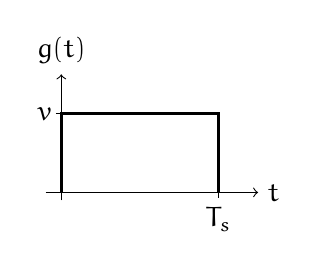
\begin{tikzpicture}
      \draw[->] (-0.2,0) -- (2.5,0) node[right] {$t$};
      \draw[->] (0,-0.1) -- (0,1.5) node[above] {$g(t)$};
      \draw[very thick] plot coordinates {(0,0) (0,1) (2,1) (2,0)};
      \draw (2,2pt) -- (2,-2pt) node[below] {$T_s$};
      \draw (-2pt,1) -- (2pt,1) node[left=2pt] {$v$};
      % \draw[very thin,color=gray] (-0.1,-0.1) grid (1.1,1.1);
    \end{tikzpicture}
    \label{fig:pulse_fr}
  }
  \subfigure[The full-response pulse used in Manchester coding]{
    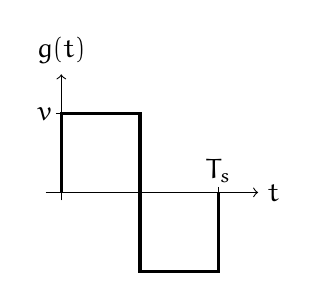
\begin{tikzpicture}
      \draw[->] (-0.2,0) -- (2.5,0) node[right] {$t$};
      \draw[->] (0,-0.1) -- (0,1.5) node[above] {$g(t)$};
      \draw[very thick] plot coordinates {(0,0) (0,1) (1,1) (1,-1) (2,-1) (2,0)};
      \draw (2,2pt) -- (2,-2pt) node[above=2pt] {$T_s$};
      \draw (-2pt,1) -- (2pt,1) node[left=2pt] {$v$};
      % \draw[very thin,color=gray] (-0.1,-0.1) grid (1.1,1.1);
    \end{tikzpicture}
    \label{fig:pulse_fr_man}
  }
  \subfigure[A partial-response filter]{
    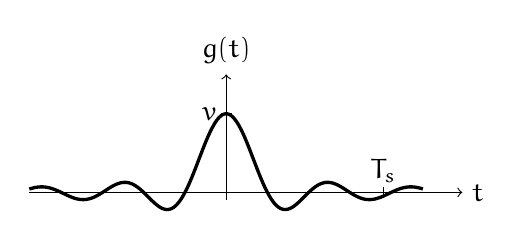
\begin{tikzpicture}[domain=-2.5:2.5]
      \draw[->] (-2.5,0) -- (3,0) node[right] {$t$};
      \draw[->] (0,-0.1) -- (0,1.5) node[above] {$g(t)$};
      \draw[very thick,smooth,samples=200,variable=\x] plot (\x,{sin(\x*6 r)/(\x*6)});
      \draw (2,2pt) -- (2,-2pt) node[above=2pt] {$T_s$};
      \draw (-2pt,1) -- (2pt,1) node[left=2pt] {$v$};
      % \draw[very thin,color=gray] (-0.1,-0.1) grid (1.1,1.1);
    \end{tikzpicture}
    \label{fig:pulse_pr}
  }
\end{figure}

Using $A_k = A_{k_i} + j A_{k_q}$, we can express $s_d(t)$ as the following sum:
\begin{equation*}
  s_d(t) = \sum_{k=-\infty}^{\infty}{A_{k_i} g(t - k T_s)} + \sum_{k=-\infty}^{\infty}{A_{k_q} g(t - k T_s)} = s_{d_i}(t) + s_{d_q}(t)
\end{equation*}
In the case of purely real symbols ($A_k \in \mathbb{R} \Rightarrow A_{k_q}=0$) the component $s_{d_q}(t)$ is zero.

For the general case, the power spectral density function of $s_d(t)$ is given by:
\begin{equation}
  \label{eq:s_d_power}
  S_d(f)=\frac{\sigma_A^2}{T_s} |G(f)|^2 + \frac{\mu_A^2}{T_s} \sum_{m=-\infty}^{\infty}{|G(f)|^2 \delta \left(f-\frac{m}{T_s}\right)}
\end{equation}
Where $G(f)$ is the fourier transform of the pulse function $g(t)$. If the symbols are symmetrically positioned around the origin, and the probabilities $p_k$ are all equal, the expectation $\mu_A$ will be zero and the second term in the above equation will be eliminated.

\begin{example}[Rectangular pulse]
  \label{ex:rect-pulse}
  If $g(t)$ is defined as a full-response rectangular pulse for the duration $T_s$, i.e.
  \begin{equation}
    \label{eq:fp-rect}
    g(t) = \left\{ \begin{array}{rl} v & t \in [0,T_s] \\
        0 &\mbox{ otherwise} \\
      \end{array} \right.
  \end{equation}
  Then the fourier transform $G(f)$ is:
  \begin{equation}
    \label{eq:fp-rect-fourier}
    G(f) = v T_s \mathrm{sinc}(\pi f T_s) e^{-j \pi f T_s}
  \end{equation}
  \begin{figure}[h!]
    \centering
    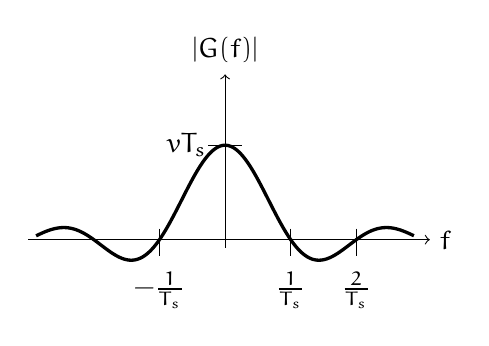
\begin{tikzpicture}[domain=-2.4:2.4]
      \draw[->] (-2.5,0) -- (2.6,0) node[right] {$f$};
      \draw[->] (0,-0.1) -- (0,2.1) node[above] {$|G(f)|$};
      \draw[very thick,smooth,samples=200,variable=\x] plot (\x,{sin(1.2*pi*\x r)/(pi*\x)});
      \draw (1/1.2,4pt) -- (1/1.2,-6pt) node[below=2pt] {$\frac{1}{T_s}$};
      \draw (-1/1.2,4pt) -- (-1/1.2,-6pt) node[below=2pt] {$-\frac{1}{T_s}$};
      \draw (2/1.2,4pt) -- (2/1.2,-6pt) node[below=2pt] {$\frac{2}{T_s}$};;
      \draw (-6pt,1.2) -- (6pt,1.2) node[left=9pt] {$v T_s$};
      % \draw[very thin,color=gray] (-0.1,-0.1) grid (1.1,1.1);
    \end{tikzpicture}
    \label{fig:fp-rect-fourier}
    \caption{$|G(f)|$ for the rectangular pulse given in Example \ref{ex:rect-pulse}}
  \end{figure}
\end{example}

Recall that the symbol rate $R_s$ and the symbol transmission time $T_s$ hold the following relation:
\begin{equation*}
  R_s = \frac{1}{T_s}
\end{equation*}

\begin{example}[BPSK]
  The BPSK encoding scheme uses the rectangular pulse from Example \ref{ex:rect-pulse}, with the two symbols $A_k \in \{-1,+1\}$. Assuming equal symbol probabilities ($p_1 = p_2 = 1/2$), we have:
  \begin{eqnarray*}
    \mu_A &=& 0 \\
    \sigma_A^2 &=& 1/2 A_1^2 + 1/2 A_2^2 = 1 \\
    S_d(f) &=& \frac{v^2T_s^2}{T_s} \mathrm{sinc}^2(\pi f T_s) = \frac{v^2}{R_s} \mathrm{sinc}^2(\frac{\pi f}{R_s})
  \end{eqnarray*}
  \begin{figure}[h!]
    \centering
    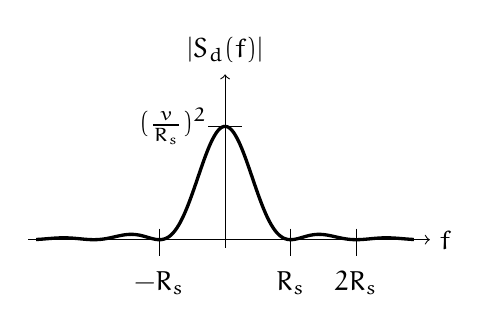
\begin{tikzpicture}[domain=-2.4:2.4]
      \draw[->] (-2.5,0) -- (2.6,0) node[right] {$f$};
      \draw[->] (0,-0.1) -- (0,2.1) node[above] {$|S_d(f)|$};
      \draw[very thick,smooth,samples=200,variable=\x] plot (\x,{(sin(1.2*pi*\x r)/(pi*\x))^2});
      \draw (1/1.2,4pt) -- (1/1.2,-6pt) node[below=2pt] {$R_s$};
      \draw (-1/1.2,4pt) -- (-1/1.2,-6pt) node[below=2pt] {$-R_s$};
      \draw (2/1.2,4pt) -- (2/1.2,-6pt) node[below=2pt] {$2R_s$};;
      \draw (-6pt,1.2^2) -- (6pt,1.2^2) node[left=9pt] {$(\frac{v}{R_s})^2$};
      % \draw[very thin,color=gray] (-0.1,-0.1) grid (1.1,1.1);
    \end{tikzpicture}
    \label{fig:fp-rect-fourier}
    \caption{$|S_d(f)|$ for BPSK}
  \end{figure}
\end{example}

\clearpage
\bibliographystyle{IEEEtran}
\bibliography{IEEEabrv,projectbib}


\end{document}


